\documentclass[handout]{beamer}
\usepackage[T1]{fontenc}
\usepackage[utf8]{inputenc}
\usepackage{lmodern}
\usepackage[italian]{babel}
\usepackage{mathrsfs}
\usepackage{cancel}

\title{Ripasso: i fenomeni elettrici}
\author{\texorpdfstring{Mattia Cozzi\newline\href{mailto:cozzimattia@gmail.com}{\texttt{cozzimattia@gmail.com}}}{Mattia Cozzi}}
\date{a.s.~2023/2024}

%\documentclass[handout]{beamer}     %usare questa classe per generare l'handout
%\usepackage{pgfpages}   %per mostrare più quadri nella stessa pagina
%\pgfpagesuselayout{4 on 1}[a4paper,border shrink=5mm,landscape]
\usetheme{Singapore}
%\useoutertheme[left]{sidebar} %elementi intorno alle diapositive
\setbeamercovered{dynamic} %modifica l'aspetto del testo grigetto delle diapositive future. Argomenti: invisible/transparent/dynamic
\usecolortheme{orchid}
%COLORE PRINCIPALE
% \definecolor{marroncino}{RGB}{156, 26, 0} % UBC Blue (primary)
% \setbeamercolor{structure}{fg=marroncino} % itemize, enumerate, etc

\theoremstyle{plain}
\newtheorem{teorema}{Teorema}

\usepackage{tikz}
\usepackage{circuitikz}

\usepackage{pgf,pgfplots,graphicx}
\usetikzlibrary{angles,quotes,arrows,shapes,decorations.markings}
\pgfplotsset{compat=1.15}
\usepgfplotslibrary{units,fillbetween} % to add units easily to axis

\newcommand{\fem}{f_{em}}

\def\angolo[#1](#2)(#3:#4:#5)% Syntax: [draw options] (center) (initial angle:final angle:radius)
    { \draw[#1] ($(#2)+({#5*cos(#3)},{#5*sin(#3)})$) arc (#3:#4:#5); }


\begin{document}

\begin{frame}
  \titlepage
\end{frame}





\begin{frame}
\frametitle{Contenuti}
\tableofcontents
\end{frame}




\section{Coulomb}

\begin{frame}
\frametitle{Carica elettrica}
Nel SI \alert<1>{la carica si misura in \emph{coulomb}}, simbolo $ C $.\pause

~

Poiché $ 1 \, C $ è una carica molto grande, spesso lavoreremo con i sottomultipli del \emph{coulomb}, in particolare:
\begin{itemize}
  \item $ 1 \, \mu C = 1 \times 10^{-6} \, C $
  \item $ 1 \, n C = 1 \times 10^{-9} \, C $
\end{itemize}\pause

~

Ogni elettrone (il \emph{quanto di carica elettrica}) ha una carica di:
\begin{center}
\colorbox{blue!30}{$ -e = - 1,6022 \times 10^{-19} \, C $}
\end{center}

Ogni carica elettrica è un multiplo (positivo o negativo) di $ e $.
\end{frame}


\begin{frame}
\frametitle{La legge di Coulomb (1)}
\begin{block}{Legge di Coulomb}
Due cariche $ q_1 $ e $ q_2 $, poste nel vuoto a distanza $ r $, esercitano l'una sull'altra una forza (attrattiva o repulsiva) di intensità:
\begin{center}
\colorbox{blue!30}{$ F = k_0 \,  \dfrac{q_1 \, q_2}{r^2} $}
\end{center}
$ k_0 = 8,99 \times 10^9 \, \frac{Nm^2}{C^2}$ =  costante elettrica del vuoto
\end{block}\pause
\begin{center}
$ k_0 = \dfrac{1}{4 \pi \varepsilon_0} $ ~~~~ con \colorbox{blue!30}{$ \varepsilon_0 = 8,854 \times 10^{-12} \,  \dfrac{C^2}{Nm^2} $}
\end{center}
\end{frame}

\begin{frame}
\frametitle{La legge di Coulomb (2)}
\begin{figure}
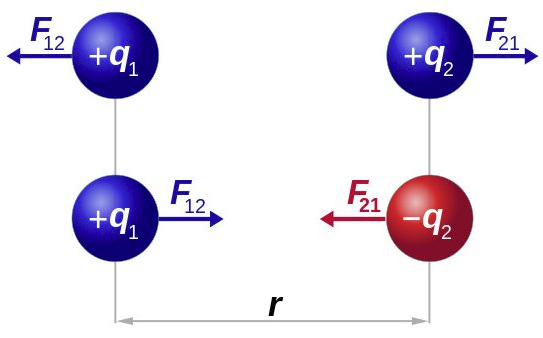
\includegraphics[width=.4\columnwidth]{img/leggecoulomb.png}
\end{figure}
Notiamo che la legge di Coulomb non fornisce direzione e verso della forza.{\pause} Essa avrà:
\begin{itemize}
  \item direzione lungo la retta che congiunge le cariche;\pause
  \item verso repulsivo per cariche dello stesso segno, attrattivo per cariche di segno opposto.
\end{itemize}
\end{frame}







\begin{frame}
\frametitle{Sovrapposizione}
Cosa succede quando una carica è sottoposta a più forze elettriche?\pause

~

\begin{block}{Principio di sovrapposizione}
La forza totale che agisce su una carica è uguale alla \alert{somma vettoriale} delle forze esercitate dalle singole cariche su di essa.
\end{block}
\visible<2>{\begin{figure}
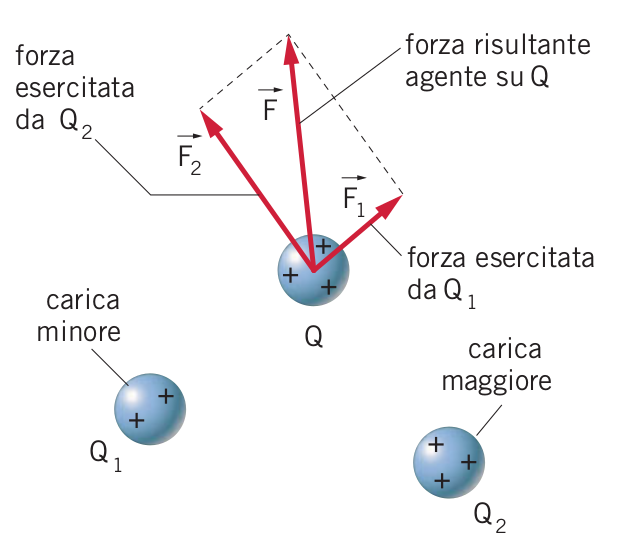
\includegraphics[width=.4\columnwidth]{img/sovrapposizionecariche.png}
\end{figure}}

\end{frame}




\begin{frame}
\frametitle{Esempio 1}
\begin{exampleblock}{Forza totale}
{\small Calcola intensità, direzione (rispetto all'orizzontale) e verso della forza totale agente su $ q_2 $.

\begin{figure}
\begin{tikzpicture}[scale=.5]
\draw (4,0) --(4,3);
\draw (0,3) --(4,3);
\node [right] at (4,1.5) {\footnotesize$ 6,0 \, mm $};
\node [above] at (2,3) {\footnotesize$ 8,0 \, mm $};
\draw [fill=blue] (0,3) circle [radius=0.1];
\node [above left] at (0,3) {\footnotesize $ q_1 = + 2,0 \, \mu C $};
\draw [fill=blue] (4,3) circle [radius=0.1];
\node [above right] at (4,3) {\footnotesize$ q_2 = + 1,0 \, \mu C $};
\draw [fill=blue] (4,0) circle [radius=0.1];
\node [below right] at (4,0) {\footnotesize$ q_3 = + 2,0 \, \mu C $};
\end{tikzpicture}
\end{figure}
}
\end{exampleblock}
\end{frame}


\begin{frame}
\frametitle{Esempio 1}
Rappresentiamo le forze agenti su $ q_2 $ e calcoliamo l'intensità delle due forze:

\begin{columns}
\begin{column}{0.3\textwidth}
\begin{figure}
\begin{tikzpicture}[scale=.5]
\draw[->,thick,red] (4,3) -- (4,6);
\draw[->,thick,cyan] (4,3) -- (6,3);
\node [below,cyan] at (5,3) {\footnotesize $ F_1 $};
\node [left,red] at (4,4.5) {\footnotesize $ F_3 $};
\draw[dashed] (4,0) --(4,3);
\node [right] at (4,1.5) {\footnotesize $ r_2 $};
\node [above] at (2,3) {\footnotesize $ r_1 $};
\draw[dashed] (0,3) --(4,3);
\draw [fill=blue] (0,3) circle [radius=0.1];
\node [above left] at (0,3) {\footnotesize $ q_1 $};
\draw [fill=blue] (4,3) circle [radius=0.1];
\node [above right] at (4,3) {\footnotesize$ q_2 $};
\draw [fill=blue] (4,0) circle [radius=0.1];
\node [below right] at (4,0) {\footnotesize$ q_3 $};
\end{tikzpicture}
\end{figure}
\end{column}
\begin{column}{0.6\textwidth}
\pause
\begin{center}
$ F_1 = k_0 \,  \dfrac{q_1 \, q_2}{r_1^2} = 2,8 \times 10^{2} \, N $

~\pause

~

$ F_3 = k_0 \,  \dfrac{q_3 \, q_2}{r_2^2} = 5,0 \times 10^{2} \, N $

~\pause

~

\colorbox{blue!30}{$ F_{tot} = (2,8)\hat{i} + (5,0)\hat{j} $}
\end{center}
\end{column}
\end{columns}

\end{frame}




\begin{frame}
\frametitle{Esempio 1}

Determiniamo l'intensità della forza totale con il TdP:
\begin{columns}
\begin{column}{0.3\textwidth}
\begin{figure}
\begin{tikzpicture}[scale=.9]
\angolo[teal,thick](4,3)(0:55:.6)
\node [above,teal] at (4.7,3.1) {\footnotesize$ \theta $};
\draw[dotted] (4,6) -- (6,6); 
\draw[dotted] (6,3) -- (6,6); 
\node [below left] at (4,3) {\footnotesize$ q_2 $};
\draw[->,thick,red!60] (4,3) -- (4,6);
\draw[->,thick,cyan!60] (4,3) -- (6,3);
\draw[->,thick,violet] (4,3) -- (6,6);
\node [below,cyan!60] at (5,3) {\footnotesize $ F_1 $};
\node [below right,violet] at (5,4.5) {\footnotesize $ F_{tot} $};
\node [left,red!60] at (4,4.5) {\footnotesize $ F_3 $};
\draw [fill=blue] (4,3) circle [radius=0.1];
\end{tikzpicture}
\end{figure}
\end{column}
\begin{column}{0.6\textwidth}
\begin{center}
$ F_{tot} = \sqrt{(F_1)^2 + (F_3)^2} = 5,7 \times 10^{2} \, N $
\end{center}
\end{column}
\end{columns}\pause
~

~

Per trovare l'angolo $ \theta $:
\begin{center}
$ \theta = \arcsin \left( \dfrac{F_3}{F_{tot}} \right) = \arccos \left( \dfrac{F_1}{F_{tot}} \right) = \arctan \left( \dfrac{F_3}{F_1} \right) = 61^{\circ} $
\end{center}
\end{frame}



\section{Campo elettrico}


\begin{frame}
\frametitle{Il concetto di campo (1)}
La forza tra due cariche è una \emph{forza a distanza}, come quella di gravità che si esercita tra due masse.

~

Come possono due corpi non in contatto interagire tra loro?\pause

~

Questa difficoltà viene superata ipotizzando che:
\begin{itemize}
  \item la presenza di una carica (massa) in un certo punto dello spazio \alert<2>{modifica le caratteristiche dello spazio} circostante;\pause
  \item un'altra carica (massa) posta nello spazio circostante \alert<3>{risente di una forza dovuta alle nuove proprietà dello spazio}.
\end{itemize}
\end{frame}


\begin{frame}
\frametitle{Il concetto di campo (2)}

\begin{figure}
\begin{tikzpicture}[scale=0.5]
\node [above,red] at (6,.1) {$ q_p $};
\draw [red, ultra thick,fill=red] (6,0) circle [radius=.1];\pause
\visible<2->{\draw [->, thick] (6,0) -- (10,0);
\node [above] at (8,0) {$ \vec{F} $};
\node [above,red] at (0,.7) {$ Q_S $};
\draw [red, ultra thick,fill=red] (0,0) circle [radius=.7];
\draw [red, ultra thick,fill=red] (6,0) circle [radius=.1];}
\end{tikzpicture}
\end{figure}
Poniamo una \emph<1>{carica di prova} (positiva e sufficientemente piccola da non modificare il sistema fisico in esame) $ q_p $ in un punto dello spazio.

~

\visible<2->{Se introduciamo una \emph<2>{carica sorgente} positiva $ Q_S $ allora \alert{$ q_p $ inizierà a sentire una forza $ \vec{F} $} dovuta alle nuove proprietà del punto in cui si trova.}
\end{frame}



\begin{frame}
\frametitle{Campo vettoriale}
Il campo elettrico (e quello gravitazionale) sono \emph{campi vettoriali}.

\begin{block}{Definizione}
\begin{columns}
\begin{column}{0.4\textwidth}
Un campo vettoriale è una funzione che ad ogni punto dello spazio associa un vettore forza.
\end{column}
\begin{column}{0.4\textwidth}
\begin{figure}
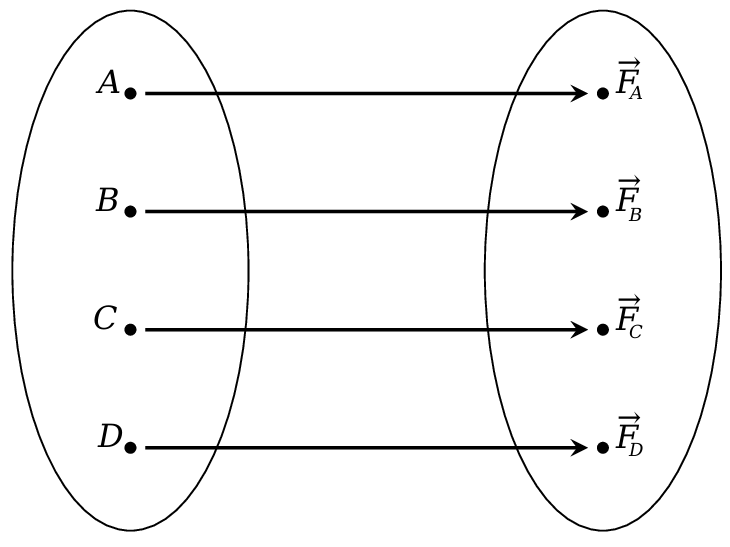
\includegraphics[width=.9\columnwidth]{img/funzionecampo.png}
\end{figure}
\end{column}
\end{columns}
\end{block}

Il vettore forza viene ottenuto con la legge di Coulomb o con quella di gravitazione universale.
\end{frame}


\begin{frame}
\frametitle{Il vettore campo elettrico}
\begin{figure}
\begin{tikzpicture}[scale=0.2]
\node [above,red] at (6,.1) {$ q_p $};
\draw [->, thick] (6,0) -- (10,0);
\node [above] at (8,0) {$ \vec{F} $};
\node [above,red] at (0,.7) {$ Q_S $};
\draw [red, ultra thick,fill=red] (0,0) circle [radius=.7];
\draw [red, ultra thick,fill=red] (6,0) circle [radius=.1];
\end{tikzpicture}
\end{figure}
Usando la nostra carica di prova $ q_p $ definiamo, per ogni punto dello spazio, il \alert{vettore campo elettrico}:

\begin{center}
\colorbox{blue!30}{$ \vec{E} = \dfrac{\vec{F}}{q_p} $}~~~~~~~~$ \left[\dfrac{N}{C}\right] $
\end{center}\pause
Notiamo che, in ogni punto dello spazio, \alert{$ \vec{E} $ è un vettore}:
\begin{itemize}
  \item con la stessa direzione e lo stesso verso di $ \vec{F} $;\pause
  \item con modulo pari a $ E = \dfrac{F}{q_p} $.
\end{itemize}
\end{frame}

\begin{frame}
\frametitle{Campo di una carica puntiforme}
In ogni punto dello spazio, possiamo calcolare il valore del campo elettrico generato da una carica sorgente $ Q_S $:
\begin{center}
$ E = \dfrac{F}{q_p} = \dfrac{k_0 \dfrac{Q_S \cancel{q_p}}{r^2}}{\cancel{q_p}} = k_0 \dfrac{Q_S }{r^2} $
\end{center}\pause
In un punto a distanza $ r $, una carica $ Q_S $ genera un campo di intensità:
\begin{center}
\colorbox{blue!30}{$ E = k_0 \dfrac{Q_S}{r^2} $}
\end{center}
\end{frame}


\begin{frame}
\frametitle{Esercizio}

  \begin{exampleblock}{Calcolo della carica sorgente}
{\small Nel vuoto, ad una distanza di $ 7,4 \, cm $ da una carica $ Q $, si misura un campo elettrico di valore $ 9,2 \times 10^{4} \, \frac{N}{C} $ rivolto verso la carica. Quanto vale $ Q $?}
\end{exampleblock}
  \pause
  Poiché il campo è rivolto verso la carica, allora $ Q $ è negativa.{\pause} Dalla formula precedente inoltre otteniamo:
  \begin{center}
  $ Q = \dfrac{Er^2}{k_0} $
  \end{center}\pause
Eseguendo i calcoli:
  \begin{center}
  $ Q = \dfrac{ \left( -9,2 \times 10^4 \, \frac{N}{C}\right) \cdot ( 7,4 \times 10^{-2} \, m)^2 }{8,99 \times10^9 \, \frac{Nm^2}{C^2}} = - 5,6 \times 10^{-8} \, C $
  \end{center}
\end{frame}





\section{Flusso}


\begin{frame}
\frametitle{Prodotto scalare}
Per poter comprendere il concetto di ``flusso di un campo'' dobbiamo ricordare il \alert<1>{prodotto scalare tra due vettori $ \vec{a} $ e $ \vec{b} $}, che si calcola come:
  \begin{center}
  $ \vec{a} \cdot \vec{b} = a b \cos\theta $
  \end{center}
  con $ \theta $ angolo tra i due vettori.\\\pause~\\
  Intuitivamente, il prodotto scalare permette di valutare ``quanto del vettore $ \vec{a} $ giace sul vettore $ \vec{b} $''.
\end{frame}


\begin{frame}
\frametitle{Vettore superficie}
\visible<1->{Introduciamo, per utilizzarlo poi nella definizione di flusso, il \emph{vettore superficie}. Data una superficie piana $ S $, esso ha:}
  \begin{itemize}
    \item \visible<2->{direzione perpendicolare a $ S $;}
    \item \visible<3->{modulo pari a $ S $.} 
  \end{itemize}
  
  \begin{figure}
\begin{tikzpicture}
\visible<1->{\fill[fill=red!20] (0,0) -- (4,0) -- (3,-1) -- (-1,-1) -- cycle;
\node [right,thick] at (2.5,0) {$ S $};}
\visible<2->{\draw [dashed] (1.5,-.5) -- (1.5,2.5);
\draw [dotted] (1.5,-1) -- (1.5,-.5);
\draw [dashed] (1.5,-1) -- (1.5,-1.5);}
\visible<3->{\node [right,blue,thick] at (1.5,1) {$ \vec{S} $};
\draw [->,blue,thick] (1.5,-.5) -- (1.5,2);}
\end{tikzpicture}
\end{figure}

\end{frame}


\begin{frame}
  \frametitle{Flusso del campo elettrico}
Il flusso del campo elettrico è definito come il prodotto scalare tra il campo elettrico $ \vec{E} $ che attraversa la superficie $ S $ e il vettore superficie $ \vec{S} $ definito sopra.
\begin{center}
   \colorbox{blue!30}{$ \Phi_{S}(\vec{E}) = \vec{E} \cdot \vec{S} = ES\cos\theta $}
\end{center}
\begin{figure}
\begin{tikzpicture}
\fill[fill=red!20] (0,0) -- (4,0) -- (3,-1) -- (-1,-1) -- cycle;
\angolo[black](1.5,-.5)(52:90:.8)
\node [left,thick] at (2.1,.6) {$ \theta $};
\node [left,blue,thick] at (1.5,1) {$ \vec{S} $};
\draw [->,blue,thick] (1.5,-.5) -- (1.5,2);
\node [left,red,thick] at (3.3,1) {$ \vec{E} $};
\draw [->,red,thick] (1.5,-.5) -- (3,1.5);
\end{tikzpicture}
\end{figure}
\end{frame}




\begin{frame}
\frametitle{Il ruolo dell'angolo}
\begin{columns}
\begin{column}{0.5\textwidth}
\begin{figure}
\begin{tikzpicture}[scale=.5]
\fill[fill=red!20] (0,0) -- (4,0) -- (3,-1) -- (-1,-1) -- cycle;
\node [right,thick] at (1.5,.3) {{\tiny $ \theta $}};
\node [left,blue,thick] at (1.5,1) {{\tiny $ \vec{S} $}};
\draw [->,blue,thick] (1.5,-.5) -- (1.5,2);
\node [right,red,thick] at (1.5,1) {{\tiny $ \vec{E} $}};
\draw [->,red,thick] (1.5,-.5) -- (1.5,1.5);
\end{tikzpicture}

$ \cos\theta = 1 $\\flusso massimo
\end{figure}


\begin{figure}
\begin{tikzpicture}[scale=.5]
\fill[fill=red!20] (0,0) -- (4,0) -- (3,-1) -- (-1,-1) -- cycle;
\angolo[black](1.5,-.5)(52:90:.8)
\node [left,thick] at (2.2,.6) {{\tiny $ \theta $}};
\node [left,blue,thick] at (1.5,1) {{\tiny $ \vec{S} $}};
\draw [->,blue,thick] (1.5,-.5) -- (1.5,2);
\node [left,red,thick] at (3.5,1) {{\tiny $ \vec{E} $}};
\draw [->,red,thick] (1.5,-.5) -- (3,1.5);
\end{tikzpicture}

$ 0 < \cos\theta < 1 $\\flusso intermedio
\end{figure}
\end{column}
\begin{column}{0.5\textwidth}
\begin{figure}
\begin{tikzpicture}[scale=.5]
\fill[fill=red!20] (0,0) -- (4,0) -- (3,-1) -- (-1,-1) -- cycle;
\angolo[black](1.5,-.5)(0:90:.8)
\node [left,thick] at (2.2,.6) {{\tiny $ \theta $}};
\node [left,blue,thick] at (1.5,1) {{\tiny $ \vec{S} $}};
\draw [->,blue,thick] (1.5,-.5) -- (1.5,2);
\node [left,red,thick] at (3.5,0) {{\tiny $ \vec{E} $}};
\draw [->,red,thick] (1.5,-.5) -- (3,-.5);
\end{tikzpicture}

$ \cos\theta = 0 $\\flusso nullo
\end{figure}



\begin{figure}
\begin{tikzpicture}[scale=.5]
\fill[fill=red!20] (0,0) -- (4,0) -- (3,-1) -- (-1,-1) -- cycle;
\angolo[black](1.5,-.5)(0:90:.8)
\angolo[black,dotted](1.5,-.5)(-45:0:.8)
\node [left,thick] at (2.2,.6) {{\tiny $ \theta $}};
\node [left,blue,thick] at (1.5,1) {{\tiny $ \vec{S} $}};
\draw [->,blue,thick] (1.5,-.5) -- (1.5,2);
\node [left,red,thick] at (3.3,-1) {{\tiny $ \vec{E} $}};
\draw [red,thick,dotted] (1.5,-.5) -- (2,-1);
\draw [->,red,thick] (2,-1) -- (2.5,-1.5);
\end{tikzpicture}

$ -1 < \cos\theta < 0 $\\flusso negativo
\end{figure}
\end{column}
\end{columns}
\end{frame}



\begin{frame}
\frametitle{Esercizio}

\begin{exampleblock}{Calcolo del flusso}
{\small Un campo elettrico uniforme di intensità $ 2,50 \times 10^4 \, \frac{N}{C} $ forma un angolo di $ 37,0^\circ $ con una superficie piana di area $ 1,53 \times 10^{-2} \, m^2 $.

Qual è il flusso del campo elettrico attraverso tale superficie?\hspace*{\fill}[$ 2,30 \times 10^{2} \, Nm^2/C $]}
\end{exampleblock}
\end{frame}



\begin{frame}
  \frametitle{Superficie chiusa}
  \begin{block}{Definizione}
    Una superficie chiusa (o gaussiana) è una superficie che racchiude un volume.
  \end{block}\pause~\\
  Sono esempi di superfici chiuse la plastica di un palloncino o le pareti di una bottiglia tappata.
\end{frame}






\begin{frame}
  \frametitle{Il teorema di Gauss per il campo elettrico}
  \begin{block}{Teorema di Gauss per il campo elettrico}
    Il flusso del campo elettrico attraverso una superficie chiusa (gaussiana) è direttamente proporzionale alla carica totale contenuta all'interno della superficie.
    \begin{center}
   \colorbox{blue!30}{$ \Phi_S (\vec{E}) = \dfrac{Q_{tot}}{\varepsilon_0} $}
   \end{center}
  \end{block}\pause
  Il valore del flusso non dipende dalla specifica superficie o da come è distribuita la carica all'interno di essa.
\end{frame}



\begin{frame}
\frametitle{Esercizio}

\begin{exampleblock}{Calcolo della carica racchiusa}
{\small Indica con $A$, $B$, $C$, $D$, $E$ e $F$ le sei facce di un cubo posto nel vuoto. Il flusso del campo elettrico attraverso ciascuna di esse è $\varphi_A = - \varphi_C = -\varphi_D = - 5,1 \times 10^3 \, \frac{Nm^2}{C}$, $\varphi_B = - \varphi_E = - 7,4 \times 10^3 \, \frac{Nm^2}{C}$ e $\varphi_F = - 3,3 \times 10^3 \, \frac{Nm^2}{C}$. Sulle superfici $A$, $B$ e $F$ il campo elettrico è rivolto verso l'interno del cubo, sulle rimanenti facce verso l'esterno.

Calcola la quantità di carica dentro la superficie cubica.}
\end{exampleblock}
\end{frame}





\section{Potenziale}

\begin{frame}
\frametitle{Forze conservative}
Sappiamo che la forza di gravità è una forza conservativa:
\begin{block}{Definizione}
Una forza si dice conservativa se il \emph{lavoro} che essa fa nello spostamento del suo punto di applicazione da un punto $ A $ fino a un punto $ B $ dipende soltanto dalle posizioni $ A $ e $ B $, ma non dal particolare percorso seguito durante lo spostamento.
\end{block}\pause
Analogamente, anche la forza di Coulomb è conservativa, e possiamo definire per essa una \alert{energia potenziale}.
\end{frame}


\begin{frame}
\frametitle{Energia potenziale di due cariche (1)}
Immaginiamo un sistema di due cariche puntiformi, $ q_1 $ e $ q_2 $, poste a distanza $ r $.
\begin{figure}
\begin{tikzpicture}[scale=0.5]
\draw [] (6,0) -- (0,0);
\node [above,red] at (6,.3) {$ q_2 $};
\draw [red, ultra thick,fill=red] (6,0) circle [radius=.3];
\node [above] at (3,0) {$ r $};
\node [above,red] at (0,.3) {$ q_1 $};
\draw [red, ultra thick,fill=red] (0,0) circle [radius=.3];
\end{tikzpicture}
\end{figure}\pause
Definiamo l'energia potenziale elettrica del sistema come:
\begin{center}
\colorbox{blue!30}{$ U(r) = k_0 \dfrac{q_1 \, q_2}{r} $}
\end{center}
\end{frame}



\begin{frame}
\frametitle{Energia potenziale di due cariche (2)}
Nella definizione precedente, abbiamo assegnato il valore $ 0 $ dell'energia potenziale alla situazione in cui le due cariche sono a distanza infinita.
\pause

~

In effetti:
\begin{center}
$ \displaystyle \lim_{r \to + \infty} k_0 \dfrac{q_1 \, q_2}{r} = 0 $
\end{center}\pause

\begin{block}{Definizione di energia potenziale elettrica}
L'energia potenziale elettrica è il lavoro compiuto dalla forza di Coulomb quando le cariche sono portate a distanza infinita tra loro.
\end{block}
\end{frame}







\begin{frame}
\frametitle{Sistema di cariche e carica di prova}
Immaginiamo un sistema formato da $ Q_1 $, $ Q_2 $ e $ Q_3 $, a cui viene avvicinata una carica di prova $ q_p $ posta nel punto $ A $.

\begin{figure}
\begin{tikzpicture}[scale=0.4]
\draw [] (8,-2) -- (-2,-2) -- (-2,5) -- (8,5) -- (8,-2);
\node [below] at (3,-2) {{\footnotesize sistema di cariche}};
\node [below,red] at (6,-.3) {$ Q_2 $};
\draw [red, ultra thick,fill=red] (6,0) circle [radius=.3];
\node [below,red] at (0,-.4) {$ Q_1 $};
\node [above,red] at (4,3.2) {$ Q_3 $};
\node [above,red] at (11,1.1) {$ q_p $};
\node [below] at (11,.9) {$ A $};
\draw [red, ultra thick,fill=red] (0,0) circle [radius=.4];
\draw [red, ultra thick,fill=red] (4,3) circle [radius=.2];
\draw [red, ultra thick,fill=red] (11,1) circle [radius=.1];
\end{tikzpicture}
\end{figure}\pause

Calcoliamo l'energia potenziale del sistema formato da $ Q_1 $, $ Q_2 $, $ Q_3 $ e $ q_p $ e indichiamola con $ U_A $.
\end{frame}


\begin{frame}
\frametitle{Potenziale elettrico}
Definiamo il potenziale elettrico $ V_A $ del punto $ A $ come:
\begin{center}
\colorbox{blue!30}{$ V_A = \dfrac{U_A}{q_p} $}
\end{center}
Il potenziale elettrico si misura in \emph{volt}: $ 1 \, V = 1 \, \dfrac{J}{C} $.\pause

~

Contrariamente a quanto possa sembrare dalla definizione, \alert<2>{il potenziale elettrico nel punto $ A $ non dipende dalla carica di prova}, ma solo dalla posizione del punto $ A $ rispetto al sistema di cariche.
\pause

~

Lo dimostriamo per un sistema semplice, formato da \alert<3>{una carica puntiforme $ Q $ e da una carica di prova $ q_p $}.
\end{frame}


\begin{frame}
\frametitle{Potenziale di una carica puntiforme}
Poniamo la carica di prova in un punto $ A $, definito dalla sua distanza $ r $ dalla carica sorgente $ Q $.
\begin{figure}
\begin{tikzpicture}[scale=0.5]
\draw [] (6,0) -- (0,0);
\node [above,red] at (6,.1) {$ q_p $};
\node [below] at (6,-.1) {$ A $};
\draw [red, ultra thick,fill=red] (6,0) circle [radius=.1];
\node [above] at (3,0) {$ r $};
\node [above,red] at (0,.3) {$ Q $};
\draw [red, ultra thick,fill=red] (0,0) circle [radius=.3];
\end{tikzpicture}
\end{figure}\pause
Calcoliamo il potenziale in $ A $:
\begin{center}
$ V(r) = \dfrac{U_A}{q_p} = \dfrac{k_0 \dfrac{Q \, \cancel{q_p} }{r}}{\cancel{q_p}} $ ~~~\pause$ \Longrightarrow  $~~~ \colorbox{blue!30}{$ V(r) = k_0 \dfrac{Q}{r} $} 
\end{center}
Notiamo che \alert<3>{tale valore non dipende da $ q_p $, ma solo dalla posizione di $ A $ rispetto a $ Q $ (cioè da $ r $)}.
\end{frame}





\begin{frame}
\frametitle{Differenza di potenziale (tensione)}

Se spostiamo la carica di prova dal punto $ A $ al punto $ B $ possiamo definire la \emph{differenza di potenziale tra $ A $ ed $ B $}:
\begin{center}
$ \Delta V_{AB} = V_B - V_A = \dfrac{U_B}{q_p} - \dfrac{U_A}{q_p} = \dfrac{\Delta U_{AB}}{q_p}$
\end{center}\pause

~

\alert{La differenza di energia potenziale} tra $ A $ e $ B $ al numeratore \alert{è il lavoro compiuto dalla forza elettrica} nello spostare la carica da $ B $ ad $ A $.
\begin{center}
\colorbox{blue!30}{$ \Delta V_{AB} = \dfrac{L_{B \to A}}{q_p} = -\dfrac{L_{A \to B}}{q_p} $}
\end{center}
\end{frame}








\begin{frame}
\frametitle{Moto spontaneo delle cariche}
Se tra i punti $ A $ e $ B $ esiste una tensione $ \Delta V $ per cui \alert{$ V_A > V_B $} (cioè il punto $ A $ è ad alto potenziale e $ B $ è a basso potenziale), avremo i seguenti moti spontanei:
\begin{figure}
\begin{tikzpicture}[scale=0.5]
\draw [->,thick,gray] (3,0) -- (5,0);
\draw [->,thick,gray] (0,0) -- (-2,0);
\draw [|-|,thick] (-6,-2) -- (9,-2);
\node [below] at (1.5,-2.3) {$ \Delta V $};
\node [above,red] at (3,.2) {$ q_+ $};
\node [below] at (-6,0) {$ A $};
\node [below] at (9,0) {$ B $};
\draw [ultra thick,fill] (-6,0) circle [radius=.1];
\draw [ultra thick,fill] (9,0) circle [radius=.1];
\draw [red, ultra thick,fill=red] (3,0) circle [radius=.2];
\node [above,blue] at (0,.2) {$ q_- $};
\draw [blue, ultra thick,fill=blue] (0,0) circle [radius=.2];
\end{tikzpicture}
\end{figure}
\end{frame}




\begin{frame}
\frametitle{Esercizio}

\begin{exampleblock}{Moto di un elettrone}
{\small Un elettrone  viene spostato da una differenza di potenziale $ \Delta V = 2,3 \times 10^5 \, V $ tra i punti $ A $ e $ B $.
\begin{itemize}
  \item Quanta energia cinetica acquista?
  \item Qual è la sua velocità finale?
\end{itemize}}
\end{exampleblock}
\pause
L'energia cinetica acquistata è il lavoro fatto dalla forza elettrica tra il punto $ B $ e il punto $ A $:
\begin{center}
$ \Delta V_{AB} = - \dfrac{L_{A \to B}}{q} $~~~ $ \Longrightarrow  $ ~~~$ \Delta K = -q \Delta V  $\pause

$ \Delta K = - (-1,60 \times 10^{-19} \, C) (2,3 \times 10 ^5 \, V) = 3,7 \times 10^{-14} \, J $
\end{center}\pause
Invertendo la formula per l'energia cinetica si trova la velocità.\hspace*{\fill}[$ 2,9 \times 10^{8} \, m/s $]
\end{frame}

\begin{frame}
\frametitle{Forza elettromotrice}
Spesso chiameremo una tensione con il nome di \alert<1>{forza elettromotrice}:\pause
\begin{enumerate}
  \item non è una forza ma una differenza di potenziale!\pause
  \item dipende dal lavoro svolto per spostare una carica $ q $ contro le forze di un campo elettrico:
  \begin{center}
  \colorbox{blue!30}{$ \fem = \dfrac{L}{q}$}
  \end{center}\pause
  \item per generatori reali (con resistenza interna) è leggermente inferiore alla tensione dichiarata.
\end{enumerate}
\end{frame}








\section{Circuitazione}



\begin{frame}
\frametitle{Campo elettrico e potenziale elettrico}
Se una carica $ q $ si muove di un vettore $ \Delta \vec{s} $ in una zona dello spazio in cui il campo elettrico $ \vec{E} $ è uniforme, allora:
\begin{center}
$ L = \vec{F} \cdot \Delta \vec{s} = q\vec{E} \cdot \Delta \vec{s} $
\end{center}\pause
Poiché $ \Delta V = - \dfrac{L}{q} $, avremo:
\begin{center}
$ \Delta V = - \dfrac{\cancel{q}\vec{E} \cdot \Delta \vec{s}}{\cancel{q}} $ \pause$~~~~~ \Longrightarrow ~~~~~  $ \colorbox{blue!30}{$ \Delta V = - \vec{E} \cdot \Delta \vec{s} $} 
\end{center}\pause
Se lo spostamento avviene parallelamente al campo, la formula precedente si riduce a:
\begin{center}
\colorbox{blue!30}{$ \Delta V = - E \Delta s $} 
\end{center}
\end{frame}




\begin{frame}
\frametitle{Concetto di circuitazione}
\begin{figure}
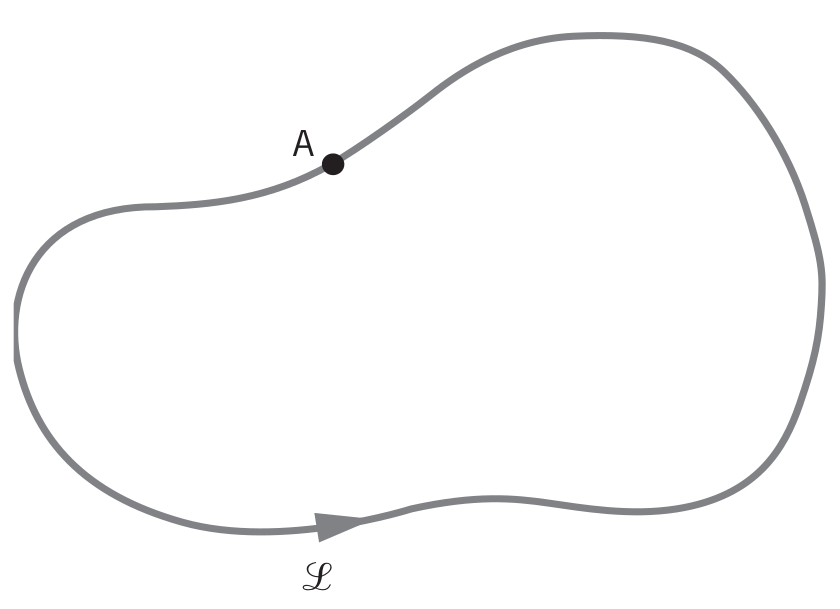
\includegraphics[width=.3\columnwidth]{img/lineachiusa.png}
\end{figure}
Quando abbiamo un campo elettrico $ \vec{E} $ che agisce in una certa zona dello spazio, risulta spesso utile valutare il suo andamento lungo una linea chiusa e orientata $ \mathscr{L} $.\pause

~

Introduciamo allora il concetto di \emph{circuitazione di un campo} lungo una linea $ \mathscr{L} $, con l'ipotesi che il campo sia costante nel tempo.
\end{frame}







\begin{frame}
  \frametitle{La circuitazione del campo elettrostatico (1)}
  Per calcolare la circuitazione del campo $ \vec{E} $ occorre scegliere arbitrariamente una linea chiusa e orientata $ \mathscr{L} $ e:\pause
  \begin{itemize}
    \item dividerla in $ n $ parti (al limite infinite) ognuna così piccola da poterla considerare \alert<2>{rettilinea} e \alert<2>{uniforme} il campo elettrico lungo di essa;\pause
    \item indicare con $ \Delta \vec{\ell}_i $ il \alert<3>{vettore spostamento} che descrive il tratto numero $ i $ di $ \mathscr{L} $;\pause
    \item determinare il vettore $ \vec{E}_i $, cioè il \alert<4>{campo elettrico lungo $ \Delta \vec{\ell}_i $};\pause
    \item calcolare il \alert<5>{prodotto scalare} $ \vec{E}_i \cdot \Delta \vec{\ell}_i $.
  \end{itemize}
\end{frame}


\begin{frame}
  \frametitle{La circuitazione del campo elettrostatico (2)}
  \begin{figure}
  \begin{tikzpicture}[xscale=.8,yscale=.8]
\draw [purple, thick] (0,0) circle [radius=3];
\angolo[black](7.5,1)(270:307:1)
\node [left, purple] at (-2.5,2) {$ \mathscr{L} $};
\draw (3,0) circle [radius=.2];
\draw (3,.2) -- (6.8,1.875);
\draw (3,-.2) -- (6.8,-1.875);
\draw (7.5,0) circle [radius=2];
\draw [thick, purple] (7.5,2)  -- (7.5,-2);
\draw [thick, blue, ->] (7.5,1)  -- (9,-1);
\node [left, purple] at (7.5,0) {{\scriptsize $ \Delta\vec{\ell}_i $}};
\node [right, blue] at (7.8,.8) {{\scriptsize $ \vec{E}_i $}};
\node [below] at (7.9,0.1) {{\scriptsize $ \theta_i $}};
\draw [thick, purple, ->] (-3,0)  -- (-3,.0001);
\end{tikzpicture}
\end{figure}
\begin{center}
   \colorbox{blue!30}{$ \Gamma_{\ell_i} (\vec{E}_i) = \vec{E}_i \cdot \Delta \vec{\ell}_i = E_i \ell_i \cos \theta_i $}
   \end{center}
\end{frame}




\begin{frame}
  \frametitle{La circuitazione lungo $ \mathscr{L} $}
  La circuitazione sarà la \alert<1>{somma di tutti i prodotti scalari}, calcolati per ogni tratto della linea $ \mathscr{L} $.
   \begin{center}
   \colorbox{blue!30}{$ \Gamma_\mathscr{L} (\vec{E}) = \sum\limits_{i=1}^n \vec{E}_i \cdot \Delta \vec{\ell}_i =  \sum\limits_{i=1}^n E_i \Delta \ell_i \cos\theta_i $}
   \end{center}
\end{frame}


\begin{frame}
  \frametitle{Il significato della circuitazione di $ \vec{E} $}
  Sappiamo che $ \vec{E}\cdot \Delta\vec{\ell} = - \Delta V $ e, indicando con $ \Delta V_i $  la differenza di potenziale tra gli estremi del segmento orientato $ \Delta \vec{\ell}_i $, avremo:
  \begin{center}
  $ \Gamma_\mathscr{L} (\vec{E}) = \sum\limits_{i=1}^n \vec{E}_i \cdot \Delta \vec{\ell}_i = \sum\limits_{i=1}^n (-\Delta V_i) = - \sum\limits_{i=1}^n \Delta V_i = 0 $
  \end{center}\pause
  La sommatoria delle differenze di potenziale lungo una linea chiusa è sempre nulla.\\\pause~\\
  
Ciò esprime matematicamente la proprietà del campo elettrostatico di essere \alert{conservativo}: il lavoro fatto dalla forza elettrica per spostare una carica non dipende dal percorso scelto ma solo dal punto di inizio e di fine (vale solo per il caso statico).
\end{frame}




\section{Corrente}





\begin{frame}
\frametitle{La corrente elettrica}
\begin{block}{Corrente elettrica}
Una corrente elettrica è un moto ordinato di cariche elettriche.
\end{block}\pause

~

\begin{block}{Intensità di corrente elettrica}
L'intensità di corrente si misura in \emph{ampere} (simbolo $A$) e vale:
\begin{center}
\colorbox{blue!30}{$ i = \dfrac{\Delta q}{\Delta t} $}~~~~~~~~\colorbox{blue!30}{$ i_{ist} = \displaystyle \lim_{\Delta t \rightarrow 0} \dfrac{\Delta q}{\Delta t} $}
\end{center}
\end{block}
\end{frame}




\begin{frame}
\frametitle{Circuito elettrico elementare}

\begin{figure}\centering
\ctikzset{bipoles/length=1.2cm}
\begin{circuitikz}[scale=0.7]
\draw (0,0) to[battery, l=$\Delta V$](6,0);
\draw (0,0) to[short, f_=$i$] (0,4);
\draw (0,4) to[R, l=R] (6,4);
\draw (6,4) to[short, f_=$i$] (6,0);
\end{circuitikz}
\end{figure}
\end{frame}




\begin{frame}
  \frametitle{La prima legge di Ohm}
  \begin{block}{Prima legge di Ohm}
Nei conduttori ohmici l'intensità di corrente è direttamente proporzionale alla differenza di potenziale applicata ai loro capi.
\begin{center}
\colorbox{blue!30}{$ i = \dfrac{\Delta V}{R} $}
\end{center}\pause
In un grafico $ \Delta V $/$ i $, la quantità $ \dfrac{1}{R} $ è il coefficiente angolare della retta.
\end{block}
  
\end{frame}




\end{document}
